%=================================%
\section{Circular benchmark}
\label{sec:circular_benchmark}
%=================================%

We start presentation of our results by demonstrating the performance of our method for the case of a circular planetary orbit with $e=0$. We benchmark our framework against many standard planet-disc interaction results, including \cite{KorycanskyPollack_1993} who used an approach identical to ours in a circular case, and present a useful point of comparison as we generalise to eccentric orbits.

% --------------------------------- %
\subsection{Numerical parameters}
\label{subsec:numerical_params}
% --------------------------------- %

To compute angular momentum characteristics of circular planet-disc coupling, we sum contributions of modes from $m_\textrm{min} = 1$ to $m_\textrm{max} = 150$. Furthermore, since $e=0$ we only need to consider the diagonal temporal contributions $l=m$. We adopt the softening parameter $b=0.3$ and consider the wake structure across a grid of typical disc power-law structures: the surface density exponent $p\in [0.0,0.5,1.0,1.5]$, the temperature exponent $q\in [0.0,0.25,0.5,0.75]$ and the disc aspect ratios $h_\textrm{p}\in[0.06,0.07,0.08,0.09,0.10]$. This range spans from uniform surface densities, to steeper profiles more typically inferred from observations. Furthermore, the temperature profile ranges from being a somewhat artificial, globally isothermal case, to a maximal temperature gradient predicted by the `lamp post' illumination model of passive disc heating \citep[see][]{Friedjung_1985}.

% --------------------------------- %
\subsection{Qualitative Wake and AMF Features}
\label{subsection:circular_wake_amf}
% --------------------------------- %

%%%%%%%%%%%%%%%%%%%%%%%%%%%%%%%%%
\begin{figure*}
    \centering
    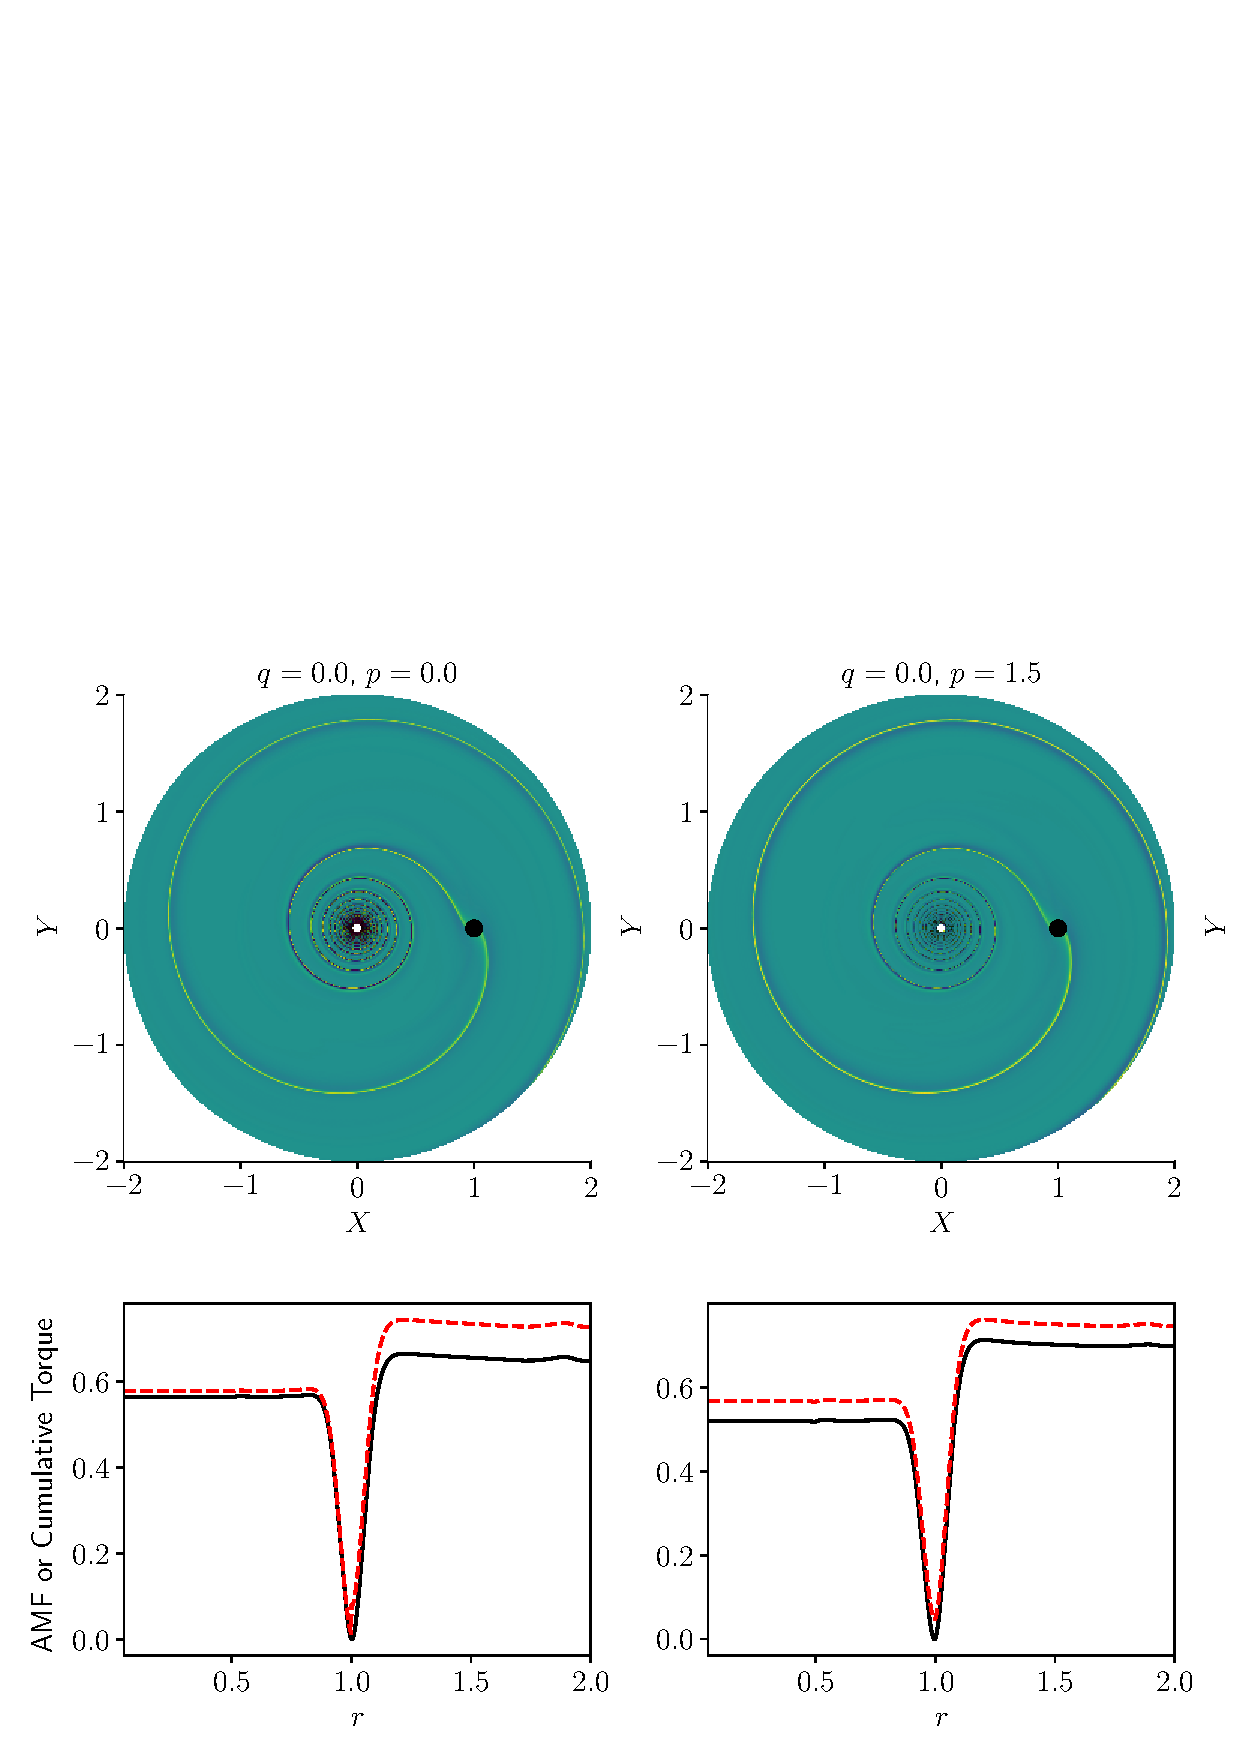
\includegraphics[width=\textwidth]{Figures/circular_morphology_torques.pdf}
    \caption{\textit{Upper panels}: The relative surface density perturbation for three different choices of $(q,p)$. From left to right (a) $= (0.0,0.0)$, (b) $= (0.0,1.5)$ and (c) $ = (0.5,1.5)$. \textit{Lower panels}: the corresponding radial torque profiles $T(r)$ (black lines) and the angular momentum flux $F_{J}(r)$ (red dashed lines) in characteristic flux units $F_{J,0}$ defined by the equation (\ref{eq:FJ0}). The inset panels zoom in to the coorbital region.}
    \label{fig:circular_morphology_torques}
\end{figure*}
%%%%%%%%%%%%%%%%%%%%%%%%%%%%%%%%%

The upper row of Fig.~\ref{fig:circular_morphology_torques} shows three example wake morphologies. Here we have specifically chosen $(q,p) = \lbrace(0.0,0.0), (0.0,1.5) , (0.5,1.5)\rbrace$ moving from left to right so as to exemplify different features in the excited AMF response ($h_\textrm{p} = 0.06$ in all cases). Notice that the relative surface density perturbation morphology for the circular planet is dominated by a single, constructive spiral arm as understood by \cite{OgilvieLubow_2003} and \citet{Rafikov2002a}, although this picture breaks down in the inner disc where multiple spiral arms emerge \citep{Bae2018,MirandaRafikov_2019a}. Only subtle qualitative differences are seen in the winding of the arm as the temperature exponent changes. 

Meanwhile more obvious differences are apparent in the corresponding integrated radial torque and AMF profiles shown in the second row. The solid black and red dashed lines plot $T(r)$ and $F_{J}(r)$, respectively, in characteristic flux units \citep{GoldreichTremaine_1980}
%
\begin{equation}
    F_{J,0} \equiv \Sigma_\textrm{p} a^4 \Omega_\textrm{p}^2 h_\textrm{p}^{-3} (M_\textrm{p}/M_*)^2.
    \label{eq:FJ0}
\end{equation}

In column (a) we consider a globally isothermal, uniform surface density disc with $q=0.0$ and $p=0.0$. We see that the net torque rises steeply away from the coorbital location as the dominant Lindblad resonances contribute to $T(r)$ within a distance of $\mathcal{O}(H)$ from the planet. Away from this region the torque levels out, although in the outer disc one may also notice small `wiggles' in both $T(r)$ and $F_J(r)$, the nature of which has recently been understood by \cite{CimermanEtAl_2024}. The difference between the plateaued torques at the inner and outer boundaries therefore provides the net torque acting back on the planet. The AMF profile exhibits a similar behaviour up to some constant offset in the outer disc region. The conservation of AMF at large distances from the planet is expected since $F_{J}$ is the wave-action for waves propagating through a globally isothermal disc \citep[see][]{MirandaRafikov_2020}. The vertical offset of $F_{J}$ from $T$ in the outer disc can be traced back to the torque exerted at the corotation resonance where there is a discontinuity in the AMF. Zooming into this region within the inset panel shows a step-wise jump whose magnitude gives the linear corotation torque (see Section \ref{subsubsec:corotation}).

In column (b) we again take a globally isothermal disc with $q = 0.0$ but this time adopt a surface density profile with $p = 1.5$. This special choice of surface density ensures that the radial vortensity gradient of the background disc is zero. Indeed, for an axisymmetric disc, the vertical component of vortensity (normal to the disc plane) is 
%
\begin{align}
\label{eq:vortensity}
    \varpi &\equiv \frac{1}{r\Sigma}\frac{\partial}{\partial r}\left(r^2 \Omega\right) \nonumber \\
    &\approx \frac{\Omega_\textrm{p}}{2\Sigma_\textrm{p}}\left[ \left(\frac{r}{a}\right)^{p-3/2}-h_\textrm{p}^2(q+p)(3/2-q)\left(\frac{r}{a}\right)^{p-q-1/2}\right],
\end{align}
%
to second order in the aspect ratio $h_\textrm{p}$. Thus, for $p=3/2$ the dominant, leading order contribution (first term) to $\varpi$ is constant with $r$. For a barotropic disc, \cite{GoldreichTremaine_1979} showed that the linear corotation torque is proportional to $\partial(\varpi^{-1})/\partial r$ evaluated at corotation; it should thus vanish for $p=3/2$ to $\mathcal{O}(h_\textrm{p})$. As a result, the zoomed inset panel in Fig.~\ref{fig:circular_morphology_torques}(b) shows no evidence of a discontinuity in the red dashed line, which is obvious in Fig.~\ref{fig:circular_morphology_torques}(a). However, there is a uniform offset between the integrated torque $T(r)$ and angular momentum flux $F_J(r)$ as previously seen by \cite{KorycanskyPollack_1993}, \cite{DongEtAl_2011} and \cite{RafikovPetrovich_2012}. Whilst the physical origin of this constant offset is not yet understood, the conservation of angular momentum still holds since $dT/dr = dF_{J}/dr$ everywhere. 

In column (c) we again take $p=1.5$ to minimize the effect of the corotation resonance. However, now we adopt a locally isothermal EoS with $q = 0.5$. In this case the torque and AMF profiles clearly do not overlap (i.e. they are not related by a constant offset) and $dT/dr \neq dF_{J}/dr$. This behaviour was noted for locally isothermal EoS by \cite{MirandaRafikov_2020} who examined the excitation and propagation of density waves for different thermal cooling prescriptions. They also showed that in the locally isothermal regime the conserved wave action is given by $F_{J}/c_s^2$ instead of $F_J$. This wave action obviously reduces to the aforementioned globally isothermal result when $c_s$ is radially constant. Keeping this phenomenology in mind will be important as we extend our results to the eccentric interaction. 


% --------------------------------- %
\subsection{Comparison with the existing literature}
\label{subsection:circular_theory}
% --------------------------------- %

Our direct numerical method circumvents the various approximations used in the past in producing analytical estimates of the torque. Here we briefly compare our methodology with previous torque prescriptions to emphasize the benefits of our approach.

We decompose the net torque into the Lindblad and corotation components in accordance with the method described in Section \ref{subsubsection:torque_computation}. Note that since we are now focusing on the case of circular planetary orbits, where only the $m=l$ modes contribute, all corotation resonances occur at the same location near $r_\mathrm{p}$ and can be extracted in one go from the single jump in the angular momentum flux profile, see Figure \ref{fig:circular_morphology_torques}(a). This is a simplification to the general pipeline where the corotation discontinuities occur at different radial locations and must be extracted separately for each modal combination before being summed together (as detailed in Section \ref{subsection:non-coorbital resonances}).

%%%%%%%%%%%%%%%%%%%%%%%%%%%%%%%%%
\begin{figure}
    \centering
    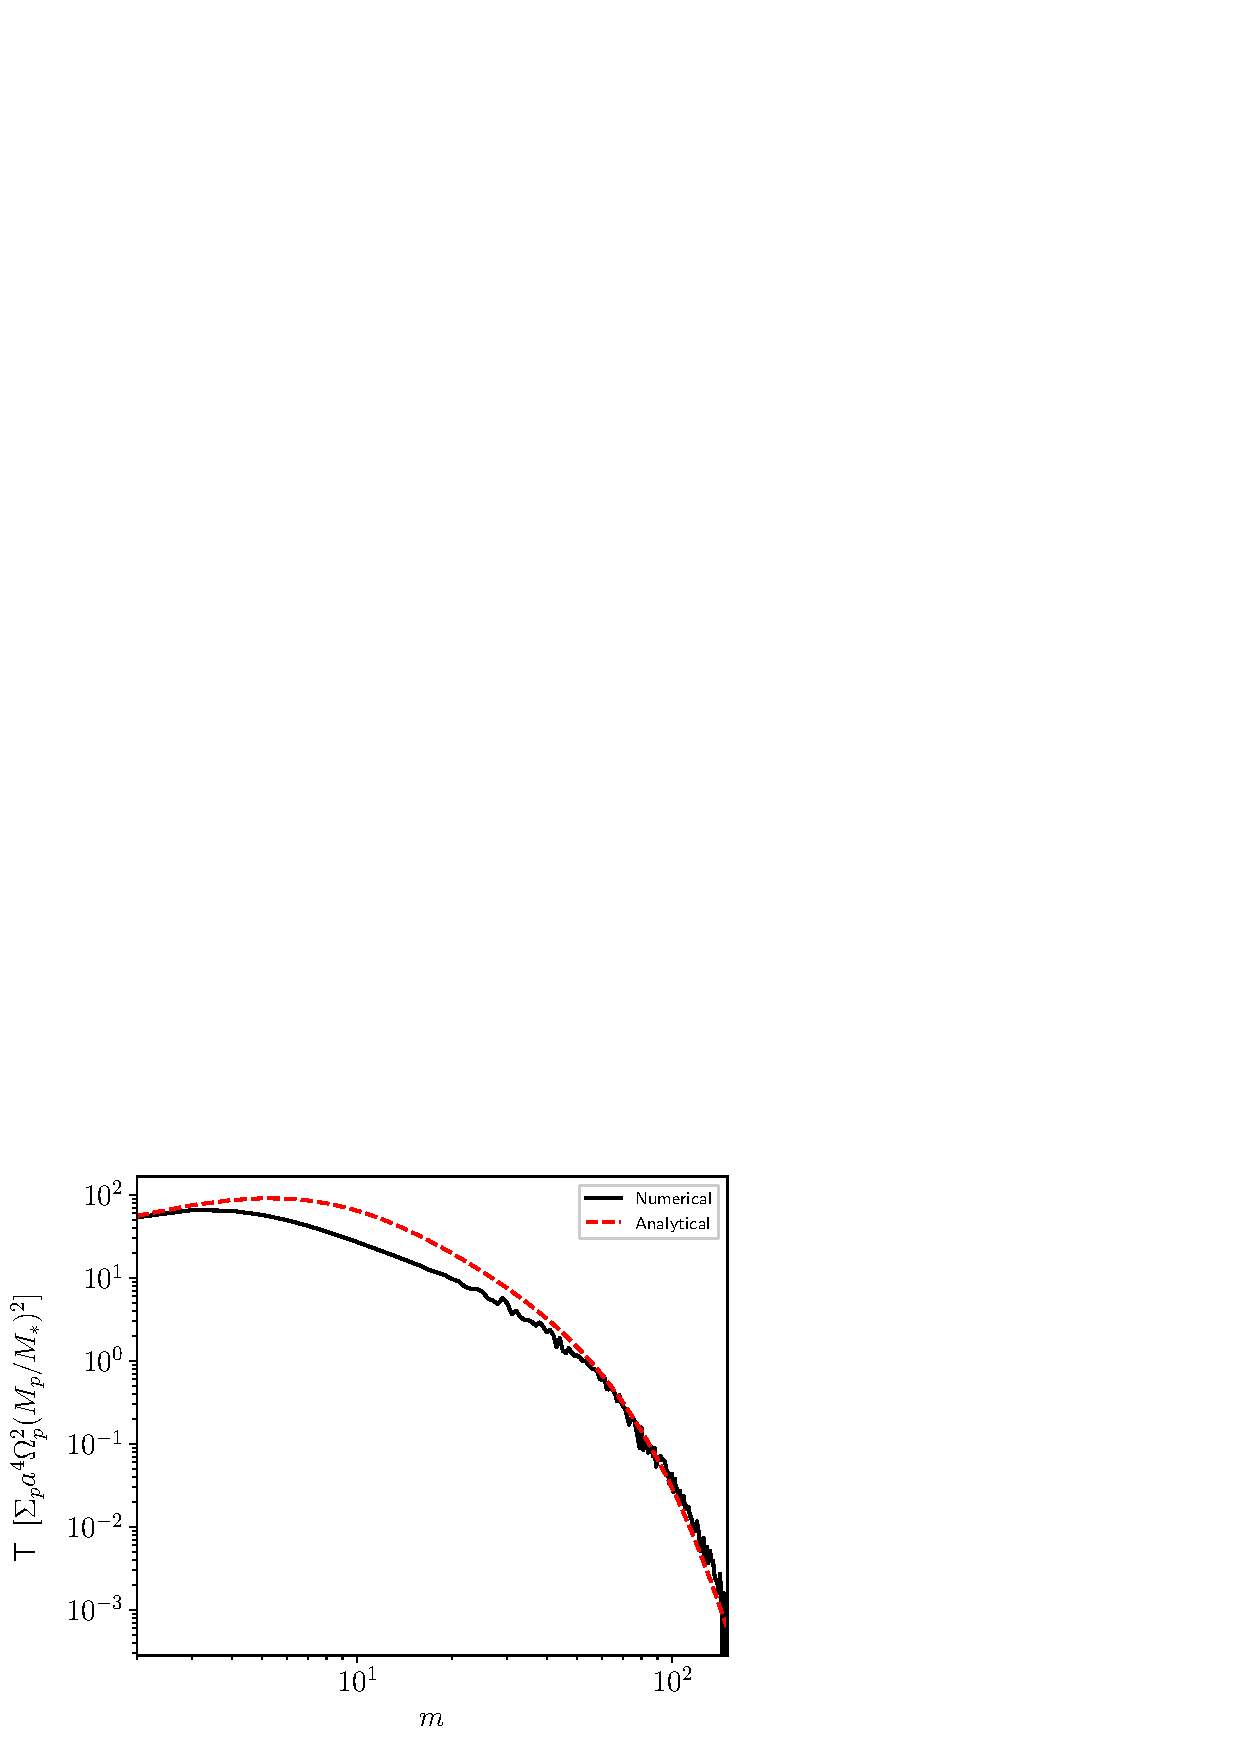
\includegraphics[width=0.9\columnwidth]{Figures/analytical_theory_torque.pdf}
    \caption{Comparison of the torque contributions as a function of the modal number $m$ for a disc with $(q,p,h,b) = (0.0,0.0,0.06,0.3)$. \textit{Red dashed line}: theoretical net Lindblad torque from equation \eqref{eq:L_WKB}. \textit{Solid black line}: numerically extracted Lindblad torque as described in the text.}
    \label{fig:analytical_theory_torque}
\end{figure}
%%%%%%%%%%%%%%%%%%%%%%%%%%%%%%%%%

In Fig.~\ref{fig:analytical_theory_torque} we show the contribution of individual modes to the net Lindblad torque for the case of $p=0.0$, $q=0.0$, $h_\mathrm{p}=0.06$ and $b=0.3$. Our results are shown as the solid black line. Notice that the dominant contributions occur for relatively small values of $m$, before experiencing the torque cut-off at larger values of $m$. We compare this numerical result with the modified WKB analytical prescription for Lindblad torques acting on the disc (dashed red curve) given by equation (26) of \cite{PapaloizouLarwood_2000},
%
\begin{align}
    \label{eq:L_WKB}
    T_{\textrm{L},\textrm{WKB}} = & \frac{S \pi^2 \Sigma}{3 \Omega \Omega_\textrm{p}} 
    \left[r\frac{d\Phi_{m}}{dr}+\frac{2 m^2 (\Omega-\Omega_\textrm{p})\Phi_{m}}{\Omega}\right]^2 \nonumber \\
    & \times \left\lbrace \frac{\left[1+m^2 c^2/(r\Omega)^2\right]^{-1/2}}{1+4m^2c^2/(r\Omega)^2}\right\rbrace ,
\end{align}
%
which is to be evaluated at the inner and outer Lindblad resonance locations where $S=-1$ and $+1$ respectively. The first part of equation \eqref{eq:L_WKB} simply corresponds to the classic result found in \cite{GoldreichTremaine_1979} whilst the multiplicative modification in the second line accounts for the pressure-induced correction introduced by \cite{Artymowicz_1993}, relevant for $m \gtrsim h_\textrm{p}^{-1}$. Whilst the two curves qualitatively agree, there are clear discrepancies within the range $m\sim 5-50$ which dominates the total torque. This echoes the findings of \cite{KorycanskyPollack_1993} who also plot the deviation between their method and analytical predictions when adopting similar disc properties. This difference highlights the benefits of using our global approach which avoid the limiting assumptions of purely analytical methods. 

It should be noted that the comparison between our results and theoretical predictions in Figure \ref{fig:analytical_theory_torque} appears qualitatively different from the similar comparison conducted by \cite{KorycanskyPollack_1993}, see their Figure 9. This might be due to the differences in the potential softening used and/or the different analytical predictions being used for comparison. For example, whilst we plot the \cite{Artymowicz_1993} modified WKB formulae at the shifted Lindblad resonances as suggested by \cite{PapaloizouLarwood_2000}, \cite{KorycanskyPollack_1993} compare their numerical results with both the cut-off modified prescription evaluated at the nominal Lindblad resonances and the unmodified \cite{GoldreichTremaine_1979} WKB expression evaluated at shifted resonance positions. 

We also explore how the full (integrated over $m$) circular torques vary with the disc properties. We demonstrate the total, Lindblad and corotation torques in Fig.~\ref{fig:circular_torques} along particular slices through the full $(q,p,h_\textrm{p})$ parameter space (outlined in Section \ref{subsec:numerical_params}). 
The upper, middle and lower rows plot the values of $T_\textrm{net}$, $T_\textrm{L}$ and $T_\textrm{C}$ respectively. Meanwhile, the first column shows the variation in torques with $q$ whilst $p=0.0$ and $h_\textrm{p}=0.06$ are held constant. Similarly, the middle column fixes $q=0.0$ and $h_\textrm{p}=0.06$ whilst p varies. Finally the last column fixes $q = 0.0$ and $p=0.0$ whilst $h_\textrm{p}$ varies. The qualitative behaviour in these slices is illustrative of the wider parameter space and the full data cube is available in the supplementary data (see Appendix \ref{app:parameter_space}). 

%%%%%%%%%%%%%%%%%%%%%%%%%%%%%%%%%
\begin{figure*}
    \centering
    \includegraphics[width=\textwidth]{Figures/circular_torques.pdf}
    \caption{The back-reaction torque (in characteristic flux units $F_{J,0}$) of the excited density wake onto the circularly orbiting planet. \textit{Upper row}: net integrated torque $T_\textrm{net}$. \textit{Middle row}: extracted Lindblad torque $T_\textrm{L}$. \textit{Lower row}: extracted corotation torque $T_C$. The columns from left to right show the variation in these quantities with disc parameters $q$, $p$ and $h_\textrm{p}$ respectively. The red crosses show the data points computed neglecting the $m=1$ mode. The black points and connective lines show the data points computed including the $m=1$ mode. The dashed blue lines show the best linear fits (\ref{eq:Tnet_fit})-(\ref{eq:TL_fit}) to the full data cube.}
    \label{fig:circular_torques}
\end{figure*}
%%%%%%%%%%%%%%%%%%%%%%%%%%%%%%%%%

The black dots and red crosses correspond to the torque values computed including and excluding the $m=1$ mode, respectively. Clearly, these values are quite different, meaning that the $m=1$ mode provides a non-negligible contribution to the torques. This might be anticipated for disc aspect ratios which are moderately thick where the torque cut-off quenches the higher order modes and therefore increases the relative importance of the lower modes. In most of the points plotted we see that the inclusion of the $m=1$ mode slightly reduces the net torque. This is because the enhancement of the negative corotation torque contribution caused by including $m=1$ mode tends to outweigh the slight increase of the Lindblad torque coming from the additional outer $m=1$ Lindblad resonance. 

It is also clear that all these torques are well fit by straight lines. More generally we perform a least squares minimisation of the three dimensional hyperplane fitting function in order to quantitatively extract these trends. We find the following fits 
%
\begin{align}
    & T_\textrm{net} = (1.413+1.109 q+1.237 p-0.017 q p)h_\textrm{p}^{1.025} F_{J,0} 
    \label{eq:Tnet_fit}\\
    & T_\textrm{L} = (2.557+2.113 q + 0.297 p -0.034 q p)h_\textrm{p}^{0.989} F_{J,0}
    \label{eq:TL_fit}
\end{align}
%
which are over-plotted as the blue dashed lines. We acknowledge that the ratio of the coefficients prepending $q$ and $p$ are notably different from those found by \cite{KorycanskyPollack_1993} in equations (32). This can be attributed to the different softening lengths being used. Whilst we adopt a softening parameter of $b = 0.3$, they use a much smaller value of $0.003$. Such a small softening leads to a sharper perturbing potential structure which cannot be easily resolved without extending the calculation to much higher values of $m$. This becomes computationally expensive for our generalised method, particularly for the eccentric case where we also have to compute off-diagonal $l \neq m$ modes. On the other hand, the larger softening length chosen here is more consistent with 2D studies of planet-disc interaction \citep[e.g.][]{CresswellNelson_2006, PaardekooperEtAl_2010} and hence is suitable for our purposes. Nonetheless, this sensitivity to parameters emphasizes the need to be careful when interpreting quantitative statements. This point is also raised by \cite{PaardekooperPapaloizou_2009} and \cite{PaardekooperEtAl_2010} who discuss that the linear dependencies on $q$ and $p$ will change depending on the choice of softening parameter $b$ and on whether the calculation is 2D or 3D. Indeed, they comment that the simple power law scaling in $b$, often tacked on to torque prescriptions, is unreliable and thus we caution against blindly using this to adjust for different softening values. As for all previous 2D planet-disc studies, our results should be regarded in the context of the region of parameter space explored. In the future we would like to extend our parameter sweep to a range of values in $b$ to investigate this effect further.